% Options for packages loaded elsewhere
\PassOptionsToPackage{unicode}{hyperref}
\PassOptionsToPackage{hyphens}{url}
\documentclass[
  ignorenonframetext,
]{beamer}
\newif\ifbibliography
\usepackage{pgfpages}
\setbeamertemplate{caption}[numbered]
\setbeamertemplate{caption label separator}{: }
\setbeamercolor{caption name}{fg=normal text.fg}
\beamertemplatenavigationsymbolsempty
% remove section numbering
\setbeamertemplate{part page}{
  \centering
  \begin{beamercolorbox}[sep=16pt,center]{part title}
    \usebeamerfont{part title}\insertpart\par
  \end{beamercolorbox}
}
\setbeamertemplate{section page}{
  \centering
  \begin{beamercolorbox}[sep=12pt,center]{section title}
    \usebeamerfont{section title}\insertsection\par
  \end{beamercolorbox}
}
\setbeamertemplate{subsection page}{
  \centering
  \begin{beamercolorbox}[sep=8pt,center]{subsection title}
    \usebeamerfont{subsection title}\insertsubsection\par
  \end{beamercolorbox}
}
% Prevent slide breaks in the middle of a paragraph
\widowpenalties 1 10000
\raggedbottom
\AtBeginPart{
  \frame{\partpage}
}
\AtBeginSection{
  \ifbibliography
  \else
    \frame{\sectionpage}
  \fi
}
\AtBeginSubsection{
  \frame{\subsectionpage}
}
\usepackage{iftex}
\ifPDFTeX
  \usepackage[T1]{fontenc}
  \usepackage[utf8]{inputenc}
  \usepackage{textcomp} % provide euro and other symbols
\else % if luatex or xetex
  \usepackage{unicode-math} % this also loads fontspec
  \defaultfontfeatures{Scale=MatchLowercase}
  \defaultfontfeatures[\rmfamily]{Ligatures=TeX,Scale=1}
\fi
\usepackage{lmodern}
\usetheme[]{Montpellier}
\ifPDFTeX\else
  % xetex/luatex font selection
\fi
% Use upquote if available, for straight quotes in verbatim environments
\IfFileExists{upquote.sty}{\usepackage{upquote}}{}
\IfFileExists{microtype.sty}{% use microtype if available
  \usepackage[]{microtype}
  \UseMicrotypeSet[protrusion]{basicmath} % disable protrusion for tt fonts
}{}
\makeatletter
\@ifundefined{KOMAClassName}{% if non-KOMA class
  \IfFileExists{parskip.sty}{%
    \usepackage{parskip}
  }{% else
    \setlength{\parindent}{0pt}
    \setlength{\parskip}{6pt plus 2pt minus 1pt}}
}{% if KOMA class
  \KOMAoptions{parskip=half}}
\makeatother
\usepackage{color}
\usepackage{fancyvrb}
\newcommand{\VerbBar}{|}
\newcommand{\VERB}{\Verb[commandchars=\\\{\}]}
\DefineVerbatimEnvironment{Highlighting}{Verbatim}{commandchars=\\\{\}}
% Add ',fontsize=\small' for more characters per line
\usepackage{framed}
\definecolor{shadecolor}{RGB}{248,248,248}
\newenvironment{Shaded}{\begin{snugshade}}{\end{snugshade}}
\newcommand{\AlertTok}[1]{\textcolor[rgb]{0.94,0.16,0.16}{#1}}
\newcommand{\AnnotationTok}[1]{\textcolor[rgb]{0.56,0.35,0.01}{\textbf{\textit{#1}}}}
\newcommand{\AttributeTok}[1]{\textcolor[rgb]{0.13,0.29,0.53}{#1}}
\newcommand{\BaseNTok}[1]{\textcolor[rgb]{0.00,0.00,0.81}{#1}}
\newcommand{\BuiltInTok}[1]{#1}
\newcommand{\CharTok}[1]{\textcolor[rgb]{0.31,0.60,0.02}{#1}}
\newcommand{\CommentTok}[1]{\textcolor[rgb]{0.56,0.35,0.01}{\textit{#1}}}
\newcommand{\CommentVarTok}[1]{\textcolor[rgb]{0.56,0.35,0.01}{\textbf{\textit{#1}}}}
\newcommand{\ConstantTok}[1]{\textcolor[rgb]{0.56,0.35,0.01}{#1}}
\newcommand{\ControlFlowTok}[1]{\textcolor[rgb]{0.13,0.29,0.53}{\textbf{#1}}}
\newcommand{\DataTypeTok}[1]{\textcolor[rgb]{0.13,0.29,0.53}{#1}}
\newcommand{\DecValTok}[1]{\textcolor[rgb]{0.00,0.00,0.81}{#1}}
\newcommand{\DocumentationTok}[1]{\textcolor[rgb]{0.56,0.35,0.01}{\textbf{\textit{#1}}}}
\newcommand{\ErrorTok}[1]{\textcolor[rgb]{0.64,0.00,0.00}{\textbf{#1}}}
\newcommand{\ExtensionTok}[1]{#1}
\newcommand{\FloatTok}[1]{\textcolor[rgb]{0.00,0.00,0.81}{#1}}
\newcommand{\FunctionTok}[1]{\textcolor[rgb]{0.13,0.29,0.53}{\textbf{#1}}}
\newcommand{\ImportTok}[1]{#1}
\newcommand{\InformationTok}[1]{\textcolor[rgb]{0.56,0.35,0.01}{\textbf{\textit{#1}}}}
\newcommand{\KeywordTok}[1]{\textcolor[rgb]{0.13,0.29,0.53}{\textbf{#1}}}
\newcommand{\NormalTok}[1]{#1}
\newcommand{\OperatorTok}[1]{\textcolor[rgb]{0.81,0.36,0.00}{\textbf{#1}}}
\newcommand{\OtherTok}[1]{\textcolor[rgb]{0.56,0.35,0.01}{#1}}
\newcommand{\PreprocessorTok}[1]{\textcolor[rgb]{0.56,0.35,0.01}{\textit{#1}}}
\newcommand{\RegionMarkerTok}[1]{#1}
\newcommand{\SpecialCharTok}[1]{\textcolor[rgb]{0.81,0.36,0.00}{\textbf{#1}}}
\newcommand{\SpecialStringTok}[1]{\textcolor[rgb]{0.31,0.60,0.02}{#1}}
\newcommand{\StringTok}[1]{\textcolor[rgb]{0.31,0.60,0.02}{#1}}
\newcommand{\VariableTok}[1]{\textcolor[rgb]{0.00,0.00,0.00}{#1}}
\newcommand{\VerbatimStringTok}[1]{\textcolor[rgb]{0.31,0.60,0.02}{#1}}
\newcommand{\WarningTok}[1]{\textcolor[rgb]{0.56,0.35,0.01}{\textbf{\textit{#1}}}}
\usepackage{longtable,booktabs,array}
\usepackage{calc} % for calculating minipage widths
\usepackage{caption}
% Make caption package work with longtable
\makeatletter
\def\fnum@table{\tablename~\thetable}
\makeatother
\usepackage{graphicx}
\makeatletter
\newsavebox\pandoc@box
\newcommand*\pandocbounded[1]{% scales image to fit in text height/width
  \sbox\pandoc@box{#1}%
  \Gscale@div\@tempa{\textheight}{\dimexpr\ht\pandoc@box+\dp\pandoc@box\relax}%
  \Gscale@div\@tempb{\linewidth}{\wd\pandoc@box}%
  \ifdim\@tempb\p@<\@tempa\p@\let\@tempa\@tempb\fi% select the smaller of both
  \ifdim\@tempa\p@<\p@\scalebox{\@tempa}{\usebox\pandoc@box}%
  \else\usebox{\pandoc@box}%
  \fi%
}
% Set default figure placement to htbp
\def\fps@figure{htbp}
\makeatother
\setlength{\emergencystretch}{3em} % prevent overfull lines
\providecommand{\tightlist}{%
  \setlength{\itemsep}{0pt}\setlength{\parskip}{0pt}}
%\documentclass[unicode,10pt]{beamer}% 'unicode'が必要
\usepackage{luatexja}% 日本語を使う場合は必須
%\usepackage[japanese]{babel}	
%\usefonttheme[onlymath]{serif}
%\usepackage[T1]{fontenc} %これを使うと、ギリシャ文字が出ない
%\usepackage{textcomp}
%\usepackage[scale=1.0]{tgheros} % Sans serif font
%\usepackage[scaled]{beramono} % Monospace font
%\usepackage{luatexja-otf}
%\renewcommand{\kanjifamilydefault}{\gtdefault}
%\usepackage[haranoaji]{luatexja-preset}

% スライド番号の表示 %%%%%%%%%%%%%%%%%%%
\makeatletter
\setbeamertemplate{footline}{%
  \leavevmode%
  \hbox{%
  \begin{beamercolorbox}[wd=.5\paperwidth,ht=2.25ex,dp=1ex,right]{date in head/foot}%
    \insertframenumber{} \hspace*{2ex} % new version without total frames
  \end{beamercolorbox}}%
  \vskip0pt%
}
\makeatother
% スライド番号の表示 %%%%%%%%%%%%%%%%%%%
\usepackage{bookmark}
\IfFileExists{xurl.sty}{\usepackage{xurl}}{} % add URL line breaks if available
\urlstyle{same}
\hypersetup{
  pdfauthor={資料作成: 田中 鮎夢},
  hidelinks,
  pdfcreator={LaTeX via pandoc}}

\title{第2章: 単回帰モデル}
\subtitle{Jeffrey Wooldridge (2016).\\
Introductory Econometrics: A Modern Approach\\
6rd ed.~Cengage Learning.}
\author{資料作成: 田中 鮎夢}
\date{2026-01-23}

\begin{document}
\frame{\titlepage}

\section{準備}\label{ux6e96ux5099}

\begin{frame}[fragile]{必要なパッケージの読み込み}
\phantomsection\label{ux5fc5ux8981ux306aux30d1ux30c3ux30b1ux30fcux30b8ux306eux8aadux307fux8fbcux307f}
\begin{itemize}
\tightlist
\item
  \texttt{wooldridge}パッケージの読み込み
\end{itemize}

\begin{Shaded}
\begin{Highlighting}[]
\FunctionTok{library}\NormalTok{(wooldridge)}
\end{Highlighting}
\end{Shaded}

\begin{itemize}
\tightlist
\item
  今回は\texttt{ggplot2}も使用してグラフを描画します（オプション）
\end{itemize}

\begin{Shaded}
\begin{Highlighting}[]
\FunctionTok{library}\NormalTok{(ggplot2)}
\end{Highlighting}
\end{Shaded}
\end{frame}

\section{2-1
単回帰モデルの定義}\label{ux5358ux56deux5e30ux30e2ux30c7ux30ebux306eux5b9aux7fa9}

\begin{frame}{単回帰モデル}
\phantomsection\label{ux5358ux56deux5e30ux30e2ux30c7ux30eb}
\begin{itemize}
\tightlist
\item
  \textbf{単回帰モデル}（simple regression model）は、2つの変数 \(x\) と
  \(y\) の関係を以下のように定義する。
\end{itemize}

\[ y = \beta_0 + \beta_1 x + u \]

\begin{itemize}
\tightlist
\item
  \(y\): \textbf{従属変数}（dependent variable）、被説明変数、目的変数
\item
  \(x\): \textbf{独立変数}（independent variable）、説明変数、共変量
\item
  \(u\): \textbf{誤差項}（error term）、撹乱項
\item
  \(\beta_0\): \textbf{切片パラメータ}（intercept parameter）
\item
  \(\beta_1\): \textbf{傾きパラメータ}（slope parameter）
\end{itemize}
\end{frame}

\begin{frame}{誤差項 \(u\) について}
\phantomsection\label{ux8aa4ux5deeux9805-u-ux306bux3064ux3044ux3066}
\begin{itemize}
\tightlist
\item
  誤差項 \(u\) は、\(y\) に影響を与える \(x\) 以外のすべての要因を表す。
\item
  単回帰分析の主な目的は、他の要因（\(u\)
  に含まれる要因）を一定に保ったまま（ceteris paribus）、\(x\) が \(y\)
  に与える効果 \(\beta_1\) を推定することである。
\item
  しかし、\(x\) と \(u\) に相関がある場合、因果関係の解釈は難しくなる。
\end{itemize}
\end{frame}

\begin{frame}{ゼロ条件付き平均の仮定}
\phantomsection\label{ux30bcux30edux6761ux4ef6ux4ed8ux304dux5e73ux5747ux306eux4eeeux5b9a}
\begin{itemize}
\tightlist
\item
  因果関係を識別するための重要な仮定は、\(x\) の値が与えられたときの
  \(u\) の平均値が0であることである。
\end{itemize}

\[ E(u|x) = 0 \]

\begin{itemize}
\tightlist
\item
  この仮定は、\(x\) と \(u\) が無相関であることを意味する。
\item
  この仮定が満たされるとき、\textbf{母回帰関数}（Population Regression
  Function: PRF）は以下のようになる。
\end{itemize}

\[ E(y|x) = \beta_0 + \beta_1 x \]
\end{frame}

\section{2-2
通常最小二乗法（OLS）の導出}\label{ux901aux5e38ux6700ux5c0fux4e8cux4e57ux6cd5olsux306eux5c0eux51fa}

\begin{frame}{OLS推定量}
\phantomsection\label{olsux63a8ux5b9aux91cf}
\begin{itemize}
\tightlist
\item
  未知のパラメータ \(\beta_0, \beta_1\) を、データの標本
  \(\{(x_i, y_i): i=1, ..., n\}\) を用いて推定する。
\item
  \textbf{残差}（residual）\(\hat{u}_i\) を以下のように定義する。
\end{itemize}

\[ \hat{u}_i = y_i - \hat{\beta}_0 - \hat{\beta}_1 x_i \]

\begin{itemize}
\tightlist
\item
  \textbf{残差二乗和}（Sum of Squared Residuals: SSR）を最小化するように
  \(\hat{\beta}_0, \hat{\beta}_1\)
  を決定する方法を\textbf{通常最小二乗法}（Ordinary Least Squares:
  OLS）と呼ぶ。
\end{itemize}

\[ \min_{\hat{\beta}_0, \hat{\beta}_1} \sum_{i=1}^n (y_i - \hat{\beta}_0 - \hat{\beta}_1 x_i)^2 \]
\end{frame}

\begin{frame}{OLS推定量の公式}
\phantomsection\label{olsux63a8ux5b9aux91cfux306eux516cux5f0f}
\begin{itemize}
\tightlist
\item
  OLS推定量 \(\hat{\beta}_1\) と \(\hat{\beta}_0\)
  は以下の式で計算される。
\end{itemize}

\[ \hat{\beta}_1 = \frac{\sum_{i=1}^n (x_i - \bar{x})(y_i - \bar{y})}{\sum_{i=1}^n (x_i - \bar{x})^2} = \frac{\text{Cov}(x, y)}{\text{Var}(x)} \]

\[ \hat{\beta}_0 = \bar{y} - \hat{\beta}_1 \bar{x} \]

\begin{itemize}
\tightlist
\item
  ここで、\(\bar{x}, \bar{y}\) はそれぞれ標本平均である。
\end{itemize}
\end{frame}

\section{2-3
Rによる単回帰分析の実装}\label{rux306bux3088ux308bux5358ux56deux5e30ux5206ux6790ux306eux5b9fux88c5}

\begin{frame}[fragile]{例: CEOの給与と自己資本利益率 (\texttt{ceosal1})}
\phantomsection\label{ux4f8b-ceoux306eux7d66ux4e0eux3068ux81eaux5df1ux8cc7ux672cux5229ux76caux7387-ceosal1}
\begin{itemize}
\tightlist
\item
  \texttt{ceosal1}
  データセットを使用して、CEOの給与（\texttt{salary}）と企業の自己資本利益率（\texttt{roe}）の関係を分析する。
\end{itemize}

\[ salary = \beta_0 + \beta_1 roe + u \]
\end{frame}

\begin{frame}[fragile]{データの確認}
\phantomsection\label{ux30c7ux30fcux30bfux306eux78baux8a8d}
\begin{Shaded}
\begin{Highlighting}[]
\CommentTok{\# データの読み込みと確認}
\FunctionTok{data}\NormalTok{(ceosal1)}
\FunctionTok{head}\NormalTok{(ceosal1[, }\FunctionTok{c}\NormalTok{(}\StringTok{"salary"}\NormalTok{, }\StringTok{"roe"}\NormalTok{)])}
\end{Highlighting}
\end{Shaded}

\begin{verbatim}
##   salary  roe
## 1   1095 14.1
## 2   1001 10.9
## 3   1122 23.5
## 4    578  5.9
## 5   1368 13.8
## 6   1145 20.0
\end{verbatim}
\end{frame}

\begin{frame}[fragile]{回帰分析の実行 (\texttt{lm}関数)}
\phantomsection\label{ux56deux5e30ux5206ux6790ux306eux5b9fux884c-lmux95a2ux6570}
\begin{itemize}
\tightlist
\item
  Rでは \texttt{lm()} 関数（Linear Model）を使用して回帰分析を行う。
\end{itemize}

\begin{Shaded}
\begin{Highlighting}[]
\CommentTok{\# 単回帰分析の実行}
\NormalTok{model\_ceo }\OtherTok{\textless{}{-}} \FunctionTok{lm}\NormalTok{(salary }\SpecialCharTok{\textasciitilde{}}\NormalTok{ roe, }\AttributeTok{data =}\NormalTok{ ceosal1)}
\end{Highlighting}
\end{Shaded}
\end{frame}

\begin{frame}[fragile]{}
\phantomsection\label{section}
\scriptsize

\begin{Shaded}
\begin{Highlighting}[]
\CommentTok{\# 結果の要約を表示}
\FunctionTok{summary}\NormalTok{(model\_ceo)}
\end{Highlighting}
\end{Shaded}

\begin{verbatim}
## 
## Call:
## lm(formula = salary ~ roe, data = ceosal1)
## 
## Residuals:
##     Min      1Q  Median      3Q     Max 
## -1160.2  -526.0  -254.0   138.8 13499.9 
## 
## Coefficients:
##             Estimate Std. Error t value Pr(>|t|)    
## (Intercept)   963.19     213.24   4.517 1.05e-05 ***
## roe            18.50      11.12   1.663   0.0978 .  
## ---
## Signif. codes:  0 '***' 0.001 '**' 0.01 '*' 0.05 '.' 0.1 ' ' 1
## 
## Residual standard error: 1367 on 207 degrees of freedom
## Multiple R-squared:  0.01319,    Adjusted R-squared:  0.008421 
## F-statistic: 2.767 on 1 and 207 DF,  p-value: 0.09777
\end{verbatim}
\end{frame}

\begin{frame}{結果の解釈}
\phantomsection\label{ux7d50ux679cux306eux89e3ux91c8}
\begin{itemize}
\tightlist
\item
  推定された回帰式は以下の通り。
\end{itemize}

\[ \widehat{salary} = 963.19 + 18.50 \cdot roe \]

\begin{itemize}
\tightlist
\item
  切片 963.19 は、\(roe=0\) のときの平均給与（千ドル）を表す。
\item
  傾き 18.50 は、\(roe\)
  が1ポイント上昇すると、給与が平均で18.5千ドル（1万8500ドル）増加することを意味する。
\end{itemize}
\end{frame}

\begin{frame}[fragile]{散布図と回帰直線のプロット}
\phantomsection\label{ux6563ux5e03ux56f3ux3068ux56deux5e30ux76f4ux7ddaux306eux30d7ux30edux30c3ux30c8}
\begin{Shaded}
\begin{Highlighting}[]
\FunctionTok{plot}\NormalTok{(ceosal1}\SpecialCharTok{$}\NormalTok{roe, ceosal1}\SpecialCharTok{$}\NormalTok{salary, }
     \AttributeTok{xlab =} \StringTok{"Return on Equity (roe)"}\NormalTok{, }
     \AttributeTok{ylab =} \StringTok{"CEO Salary (salary)"}\NormalTok{,}
     \AttributeTok{main =} \StringTok{"CEO Salary vs ROE"}\NormalTok{)}
\FunctionTok{abline}\NormalTok{(model\_ceo, }\AttributeTok{col =} \StringTok{"blue"}\NormalTok{, }\AttributeTok{lwd =} \DecValTok{2}\NormalTok{)}
\end{Highlighting}
\end{Shaded}

\pandocbounded{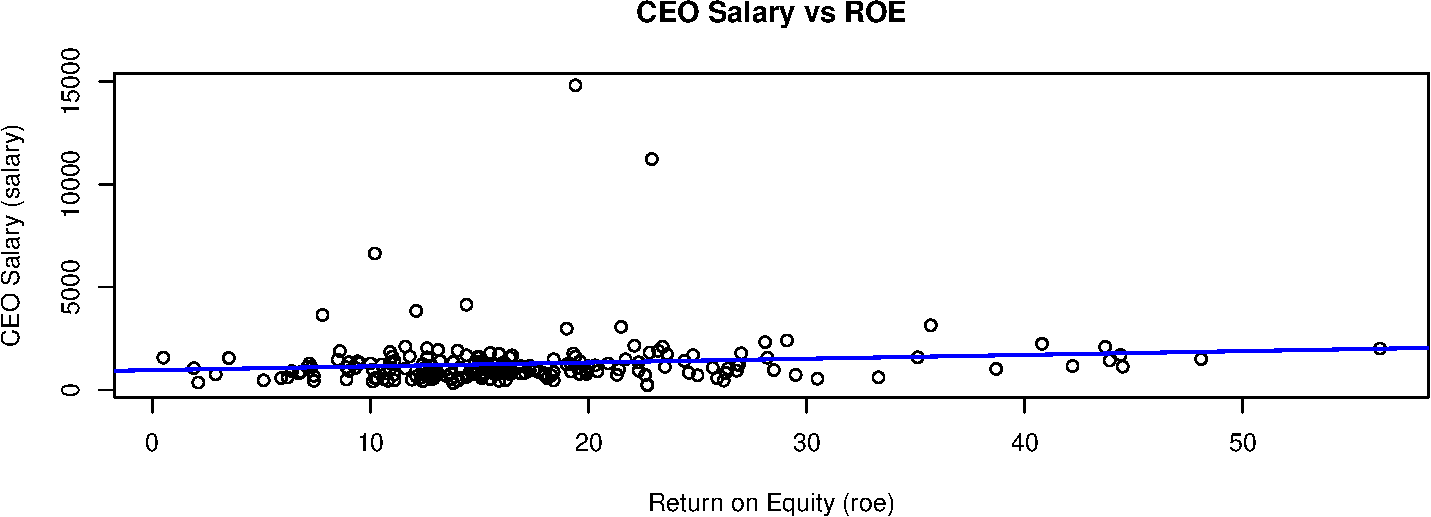
\includegraphics[keepaspectratio]{Wooldridge02_files/figure-beamer/unnamed-chunk-4-1.pdf}}
\end{frame}

\section{2-4
適合度と決定係数}\label{ux9069ux5408ux5ea6ux3068ux6c7aux5b9aux4fc2ux6570}

\begin{frame}{決定係数 (\(R^2\))}
\phantomsection\label{ux6c7aux5b9aux4fc2ux6570-r2}
\begin{itemize}
\tightlist
\item
  \textbf{決定係数}（R-squared）は、従属変数の変動のうち、独立変数によって説明される割合を示す。
\end{itemize}

\[ R^2 = \frac{\text{SSE}}{\text{SST}} = 1 - \frac{\text{SSR}}{\text{SST}} \]

\begin{itemize}
\item
  SSE (Explained Sum of Squares): 回帰変動
\item
  SSR (Residual Sum of Squares): 残差変動
\item
  SST (Total Sum of Squares): 全変動
\item
  \(0 \le R^2 \le 1\)
  であり、1に近いほどモデルの当てはまりが良いとされるが、低いからといってモデルが無意味なわけではない。
\end{itemize}
\end{frame}

\begin{frame}[fragile]{\texttt{ceosal1} の \(R^2\)}
\phantomsection\label{ceosal1-ux306e-r2}
\begin{itemize}
\tightlist
\item
  先ほどの分析結果（\texttt{summary(model\_ceo)}）を見ると、\texttt{Multiple\ R-squared:\ \ 0.01319}
  となっている。
\item
  これは、CEOの給与の変動の約1.3\%しか \texttt{roe}
  で説明できていないことを意味する。
\item
  給与には \texttt{roe} 以外の多くの要因が影響していることが示唆される。
\end{itemize}
\end{frame}

\section{2-5
関数形：対数を用いたモデル}\label{ux95a2ux6570ux5f62ux5bfeux6570ux3092ux7528ux3044ux305fux30e2ux30c7ux30eb}

\begin{frame}{対数モデルの利点}
\phantomsection\label{ux5bfeux6570ux30e2ux30c7ux30ebux306eux5229ux70b9}
\begin{itemize}
\tightlist
\item
  変数を対数変換（log）することで、非線形な関係を線形モデルとして扱うことができる。
\item
  係数の解釈が「変化量」から「変化率（\%）」に変わる。
\end{itemize}

\begin{longtable}[]{@{}
  >{\raggedright\arraybackslash}p{(\linewidth - 4\tabcolsep) * \real{0.1188}}
  >{\raggedright\arraybackslash}p{(\linewidth - 4\tabcolsep) * \real{0.3762}}
  >{\raggedright\arraybackslash}p{(\linewidth - 4\tabcolsep) * \real{0.5050}}@{}}
\toprule\noalign{}
\begin{minipage}[b]{\linewidth}\raggedright
モデル
\end{minipage} & \begin{minipage}[b]{\linewidth}\raggedright
方程式
\end{minipage} & \begin{minipage}[b]{\linewidth}\raggedright
解釈
\end{minipage} \\
\midrule\noalign{}
\endhead
Level-level & \(y = \beta_0 + \beta_1 x\) &
\(\Delta y = \beta_1 \Delta x\) \\
Log-level & \(\log(y) = \beta_0 + \beta_1 x\) &
\(\% \Delta y \approx (100 \beta_1) \Delta x\) \\
Level-log & \(y = \beta_0 + \beta_1 \log(x)\) &
\(\Delta y \approx (\beta_1 / 100) \% \Delta x\) \\
Log-log & \(\log(y) = \beta_0 + \beta_1 \log(x)\) &
\(\% \Delta y \approx \beta_1 \% \Delta x\) (弾力性) \\
\bottomrule\noalign{}
\end{longtable}
\end{frame}

\begin{frame}[fragile]{例: 賃金方程式 (\texttt{wage1})}
\phantomsection\label{ux4f8b-ux8cc3ux91d1ux65b9ux7a0bux5f0f-wage1}
\begin{itemize}
\tightlist
\item
  賃金（\texttt{wage}）の対数をとり、教育年数（\texttt{educ}）で回帰する（Log-levelモデル）。
\end{itemize}

\[ \log(wage) = \beta_0 + \beta_1 educ + u \]

\begin{Shaded}
\begin{Highlighting}[]
\FunctionTok{data}\NormalTok{(wage1)}
\CommentTok{\# 対数賃金の回帰分析}
\NormalTok{model\_wage }\OtherTok{\textless{}{-}} \FunctionTok{lm}\NormalTok{(}\FunctionTok{log}\NormalTok{(wage) }\SpecialCharTok{\textasciitilde{}}\NormalTok{ educ, }\AttributeTok{data =}\NormalTok{ wage1)}
\end{Highlighting}
\end{Shaded}
\end{frame}

\begin{frame}[fragile]{}
\phantomsection\label{section-1}
\scriptsize

\begin{Shaded}
\begin{Highlighting}[]
\FunctionTok{summary}\NormalTok{(model\_wage)}\SpecialCharTok{$}\NormalTok{coefficients}
\end{Highlighting}
\end{Shaded}

\begin{verbatim}
##               Estimate  Std. Error  t value     Pr(>|t|)
## (Intercept) 0.58377267 0.097335834  5.99751 3.736702e-09
## educ        0.08274437 0.007566694 10.93534 3.270645e-25
\end{verbatim}
\end{frame}

\begin{frame}{結果の解釈（賃金方程式）}
\phantomsection\label{ux7d50ux679cux306eux89e3ux91c8ux8cc3ux91d1ux65b9ux7a0bux5f0f}
\[ \widehat{\log(wage)} = 0.584 + 0.083 \cdot educ \]

\begin{itemize}
\tightlist
\item
  \(\beta_1 = 0.083\)
\item
  これは、教育年数が1年増えると、賃金が約 \(8.3\%\)
  増加することを意味する（\textbf{教育の収益率}）。
\item
  \(100 \times 0.083 = 8.3\%\)
\end{itemize}
\end{frame}

\section{まとめ}\label{ux307eux3068ux3081}

\begin{frame}{まとめ}
\phantomsection\label{ux307eux3068ux3081-1}
\begin{itemize}
\tightlist
\item
  単回帰モデルは、2変数間の線形関係を分析する基本的な手法である。
\item
  OLS（最小二乗法）は、残差二乗和を最小化することでパラメータを推定する。
\item
  \(R^2\)（決定係数）はモデルの当てはまりの良さを測る指標である。
\item
  対数変換を用いることで、弾力性や成長率（\%変化）として係数を解釈できる。
\end{itemize}
\end{frame}

\end{document}
